\chapter{Casi di studio e valutazioni}
\noindent In questa sezione verranno riportati i casi studio e i test effettuati sul framework. Tutti questi casi studio sono stati eseguiti su un sistema HPC Galielo-100 Cineca con le specifiche riportate nella tabella sotto

\vspace{.7cm}
\begin{center}

\begin{tabular}{l|l}
    \hline
    \textbf{Parameter} & \textbf{Value} \\
    \hline
    Number of nodes used & 3 \\
    \hline
    Processor & Intel CascadeLake 8260 \\
    \hline
    Number of sockets per node & 2 \\
    \hline
    Number of cores per socket & 24 \\
    \hline
    Memory size per node & 384 GB \\
    \hline
    Interconnect & Mellanox Infiniband 100GbE \\
    \hline
    OS & CentOS Linux \\ 
    \hline
    MPI & Open MPI  4.1.1 \\
    \hline
\end{tabular}
\end{center}
\section{Sincronizzazione orologi su nodi diversi}
Per ottenere risultati attendibili sulla metrica del tempo è stato necessario sincronizzare i nodi utilizzati prima di poter far partire i test. Per farlo è stato necessario implementare delle MPI\_Barrier dopo il quale una \emph{clock\_getTime(MONOTONIC)} per più volte, andando successivaemtene a ripulire ed elaborare i dati riportati.

\begin{figure}
    \centering
    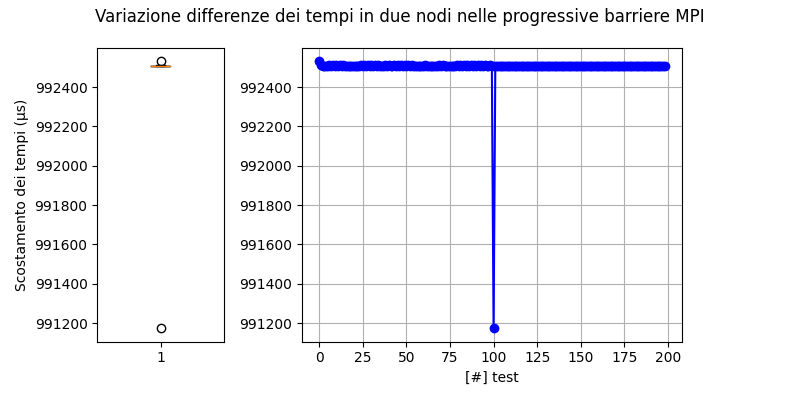
\includegraphics[width=\textwidth]{./results/time_sync_node.png}
    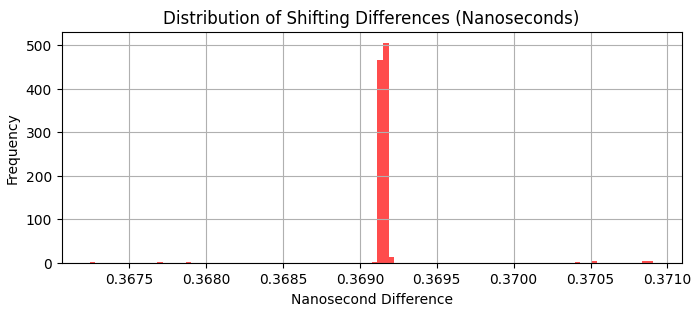
\includegraphics[width=\textwidth]{./results/time_sync_distribution.png}
\end{figure}

\section{Test}

\section{Risultati}

\section{Modello}

\section{Scheletro componenti}